\documentclass[11pt, twoside, pdftex]{article}

% This include all the settings that we should use for the document
\newcommand{\PDFTitle}{Introduction to Nios\textsuperscript{\textregistered} V}
\newcommand{\commonPath}{../../Common}
\newcommand{\datePublished}{Mar 2022}

\newcommand{\versnum}{21.1} %version number quartus/AMP
\newcommand{\quartusname}{Quartus\textsuperscript{\textregistered} Prime}	
\newcommand{\textBar}{For \quartusname{} \versnum{}}
\newcommand{\thisyear}{2022 } %for copyright
\newcommand{\company}{FPGAcademy.org}
\newcommand{\longteamname}{FPGAcademy.org}
\newcommand{\teamname}{FPGAcademy}
\newcommand{\website}{FPGAcademy.org}

\newcommand{\productAcronym}{AMP}
\newcommand{\productNameShort}{Monitor Program}

\newcommand{\productNameMedTM}{Monitor Program}
\newcommand{\productNameMed}{Monitor Program}

%\newcommand{\headerLogoFilePath}[1]{#1/FPGAcademy.png}



\setlength\topmargin{-0.25in}
\setlength\headheight{0in}
\setlength\headsep{0.35in}
\setlength\textheight{8.5in}
\setlength\textwidth{7in}
\setlength\oddsidemargin{-0.25in}
\setlength\evensidemargin{-0.25in}
\setlength\parindent{0.25in}
\setlength\parskip{0in} 

\pdfpagewidth 8.5in
\pdfpageheight 11in

\input{\commonPath/Docs/listingsstyles}

%\usepackage[centering]{geometry}.
%%%%%%%%%%%%%%%%%%%%%%%%%%%%%%%%%%%%%%%%%%%%%%%%%%%
% Document Settings
\usepackage[labelsep=period]{caption}
% we can choose a better font later
%\usepackage{palatino}
\usepackage{fourier}
%\fontencoding{T1}
% include common used symbols
\usepackage{textcomp}
% add support for graphics
\usepackage{graphicx}
\usepackage[usenames, dvipsnames]{color}
% enable to draw thick or thin table hlines
\setlength{\doublerulesep}{\arrayrulewidth}
\usepackage{longtable}
\setlongtables
%\usepackage{array}
% It may be better to use PDFLaTeX as it can generate bookmarks for the
% document

% Add some useful packages
\usepackage{ae,aecompl}
\usepackage{epsfig,float,times}

% reset the font for section
\usepackage{sectsty}
%\allsectionsfont{\fontfamily{ptm}\selectfont}
\allsectionsfont{\usefont{OT1}{phv}{bc}{n}\selectfont}

% use compact space for sections
\usepackage[compact]{titlesec}
\titlespacing{\section}{0pt}{0.2in}{*0}
\titlespacing{\subsection}{0pt}{0.1in}{*0}
\titlespacing{\subsubsection}{0pt}{0.05in}{*0}

% fancyhdr header and footer customization
\usepackage{layout}
\usepackage{fancyhdr}
\pagestyle{fancy}
\fancyhead{}
\fancyhead[R]{\textit{\tiny{\textBar}}}
\fancyfoot{}
\fancyfoot[LO,
RE]{\textrm{\href{https://www.fpgacademy.org}{\small \longteamname}} \\ {\small \datePublished }}
\fancyfoot[RO, LE]{\small \thepage}
% two-side settings
%\fancyhead{} % clear all header fields
%\fancyfoot{} % clear all footer fields
%\fancyfoot[LE,RO]{\thepage}
\renewcommand{\headrulewidth}{2pt}
\renewcommand{\headrule}{{\color{blue} \hrule width\headwidth height\headrulewidth \vskip-\headrulewidth}}
\renewcommand{\footrulewidth}{0pt}

% Format the footer on page 1
\fancypagestyle{plain}{
\fancyhead{}
\fancyfoot{}
\fancyfoot[LO,
RE]{\textrm{\href{https://www.fpgacademy.org}{\small \longteamname}} \\ {\small \datePublished }}
\fancyfoot[RO, LE]{\small \thepage}
\renewcommand{\headrulewidth}{0pt}
}
% adjust some setting to try to make the figure stay in the same page with text
% Reference: 	http://www.cs.uu.nl/~piet/floats/node1.html
%   			http://mintaka.sdsu.edu/GF/bibliog/latex/floats.html
%   General parameters, for ALL pages:
\renewcommand{\topfraction}{0.9}	% max fraction of floats at top
\renewcommand{\bottomfraction}{0.8}	% max fraction of floats at bottom
%   Parameters for TEXT pages (not float pages):
\setcounter{topnumber}{3}
\setcounter{bottomnumber}{3}
\setcounter{totalnumber}{5}     % 2 may work better
\setcounter{dbltopnumber}{2}    % for 2-column pages
\renewcommand{\dbltopfraction}{0.9}	% fit big float above 2-col. text
\renewcommand{\textfraction}{0.07}	% allow minimal text w. figs
%   Parameters for FLOAT pages (not text pages):
\renewcommand{\floatpagefraction}{0.7}	% require fuller float pages
% N.B.: floatpagefraction MUST be less than topfraction !!
\renewcommand{\dblfloatpagefraction}{0.7}	% require fuller float pages
%%%%%%%%%%%%%%%%%%%%%%%%%%%%%%%%%%%%%%%%%%%%%%%%%%%
% remember to use [htp] or [htpb] for placement
%%%%%%%%%%%%%%%%%%%%%%%%%%%%%%%%%%%%%%%%%%%%%%%%%%%

% set no indent for paragraph
\setlength{\parindent}{0em}
\addtolength{\parskip}{11pt}
\newcommand{\compact}{[topsep=0pt]}
% use this package to reduce space
\usepackage{enumitem}
\usepackage{multirow}
\usepackage{rotating}
\usepackage{pifont}
\usepackage{dingbat}
\newcommand{\itemsecond}{$\circ$}
%
%%%%%%%%%%%%%%%%%%
\date{}
\author{}
%%%%%%%%%%%%%%%%%%
\newcommand{\de}{DE-series}
\newcommand{\up}{FPGAcademy}
\newcommand{\fabric}{Avalon Switch Fabric}
\newcommand{\TODO}[1]{\textcolor{red}{\textbf{TODO}: #1}}
\def\registered{{\ooalign{\hfil\raise .00ex\hbox{\scriptsize R}\hfil\crcr\mathhexbox20D}}}

% enable url and reference(bookmarks) in pdf
\usepackage{url}
\usepackage[pdftex, colorlinks]{hyperref}
\hypersetup{%
pdftitle={\PDFTitle},
linkcolor=blue,
hyperindex=true,
pdfauthor={\longteamname},
pdfkeywords={FPGAcademy, Academic Program, Example System},
bookmarksnumbered,
bookmarksopen=false,
filecolor=blue,
pdfstartview={FitH},
urlcolor=blue,
plainpages=false,
pdfpagelabels=true,
linkbordercolor={1 1 1} %no color for link border
}%
%%%%%%%%%%%%%%%%%%%%%%%%%%%%%%%%%%%%%%%%%%%%%%%%%%%
\setlength{\fboxsep}{0.7pt}
\setlength{\fboxrule}{0.5pt}



%%%%%%%%%%%%%%%%%%%%%%%%%
% Add title
\newcommand{\doctitle}{Introduction to Nios\textsuperscript{\textregistered} V}
\newcommand{\dochead}{Introduction to Nios\textsuperscript{\textregistered} V}
% Usually no need to change these two lines
\title{\fontfamily{phv}\selectfont{\doctitle} }
\chead{ \small{\textsc{\bfseries \dochead} } }
% Customizations
\newenvironment{ctabbing}%
{\begin{center}\begin{minipage}{\textwidth}\begin{tabbing}}
{\end{tabbing}\end{minipage}\end{center}}

%%%%%%%%%%%%%%%%%%%%%%%%%
% Allows multiple figures per page

\renewcommand\floatpagefraction{.9}
\renewcommand\topfraction{.9}
\renewcommand\bottomfraction{.9}
\renewcommand\textfraction{.1}   
\setcounter{totalnumber}{50}
\setcounter{topnumber}{50}
\setcounter{bottomnumber}{50}
\raggedbottom

%%%%%%%%%%%%%%%%%%
%%% DOCUMENT START
%\begin{document}
\begin{document}
\begin{table}
    \centering
    \begin{tabular}{p{5cm}p{4cm}}
        \hspace{-3cm}
        &
        \raisebox{1\height}{\parbox[h]{0.5\textwidth}{\Large\fontfamily{phv}\selectfont{\textsf{\doctitle}}}}
    \end{tabular}
    \label{tab:logo}
\end{table}

\colorbox[rgb]{0,0.384,0.816}{\parbox[h]{\textwidth}{\color{white}\textsf{\textit{\textBar}}}}

\thispagestyle{plain}
 
\section{Introduction}

This tutorial presents an introduction to the Altera\textsuperscript{\textregistered}
{\it Nios}\textsuperscript{\textregistered} {\it V} processor, 
which is an implementation of the RISC-V processor architecture. Three versions of 
Nios~V exist, each with different features and capabilities.  Documentation for each 
of the three versions, designated by suffices {\it /c}, {\it /m}, and {\it /g}, 
can be found by searching on the Internet for keywords such as \texttt{Nios~V versions}.

This document is intended for a reader who is using a Nios~V computer system on one of 
the DE-series boards that are described in the \texttt{Teaching and Projects Boards} 
section of the {\small \href{https://www.fpgacademy.org/boards.html} {FPGAcademy.org}} website. 
Thus, we focus on the version of the processor that are included in those computer
systems, which are Nios~V/m or Nios~V/g. 

{\bf Contents}:
\begin{itemize}
\item Nios~V System
\item Overview of Nios~V Processor Features
\item Register Structure
\item Accessing Memory and I/O Devices
\item Addressing
\item Instruction Set
\item Assembler Directives
\item Example Program
\item Exception and Interrupt Processing
\item Nios~V Internal Timer
\end{itemize}
\clearpage
\newpage

\section{Background}

Nios~V is a soft processor, defined in a hardware description language,
which can be implemented in an Altera FPGA devices by using the 
Quartus Prime CAD system. 
In this tutorial we assume that the reader is using Nios~V as part of a computer system
that is implemented on a DE1-SoC board. If another DE-series board is used, then most of
the discussion will still be applicable, but some features of the computer system might 
be different.

\section{Nios~V System}
The Nios~V processor can be used with a variety of other components to form 
a computer system. One example of such a system is shown in Figure~\ref{fig:system}.
It is called the {\it DE1-SoC Computer with Nios~V}, and is implemented on a DE1-SoC board. 
A complete description of this system, describing all of the peripherals connected to
Nios~V, is available as part of the \texttt{Computer Organization} section of the
\texttt{Courses} tab on 
{\small \href{https://www.fpgacademy.org/courses.html} {FPGAcademy.org}}. 
\footnote{This computer system also includes an ARM A9 processor subsystem. It is 
described in the document entitled {\it DE1-SoC Computer System with ARM* Cortex* A9},
which is available on the 
{\small \href{https://www.fpgacademy.org/tutorials.html} {FPGAcademy.org}} website.}
 
\begin{figure}[H]
   \begin{center}
      \includegraphics[scale=0.85]{figures/Nios_V_system.pdf}
   \caption{A Nios~V system implemented on a DE1-SoC board.} 
	 \label{fig:system}
	 \end{center}
\end{figure}

\newpage
\section{Nios\textsuperscript{\textregistered} V Processor Architecture}

Nios~V is based on the RISC-V processor architecture that is described in detail on
the {\small \href{https://www.riscv.org} {riscv.org}} website. Useful information for
programmers using RISC-V can be found on the 
{\small \href{https://five-embeddev.com} {five-embeddev.com}} website.
Using the terminology from the RISC-V specification, Nios~V has features in
the {\it RV32IMZicsr} architecture. This mnemonic denotes a 32-bit processor that supports 
integer computations ({\it 32I}) including multiply and divide ({\it M}, available in
Nios~V/g), with special instructions that are used for control purposes ({\it Zicsr}). 

\section{Register Structure}
\label{sec:registers}

All registers in Nios~V are 32-bits long. There are 32 general-purpose registers, 
{\it x0} to {\it x31}, plus a program counter, {\it pc}. The general-purpose registers
are listed in Figure~\ref{fig:gp_regs} 
and are used for performing integer computations in program code. 

Register {\it x0} is referred to as the {\it zero} register.  It always contains the 
constant 0. Thus, reading this register returns the value 0, while writing to it has no effect.  

Most of the other general-purpose registers can be used interchangeably in practice. However, 
by convention software programs usually treat the registers in a particular way, as indicated
below:

\begin{itemize}
\item Registers {\it x1} is known as the {\it ra} register, because it is often used
to hold the {\it return address} from a subroutine. 
\item Register {\it x2} is known as the {\it sp} register, because it is typically used 
as the {\it stack pointer}. 
\item Registers {\it x3} and {\it x4} are used as special pointer registers by compilers
for high-level languages. These registers are referred to as the {\it global} and 
{\it thread} pointers, respectively. 
\item Registers {\it x5} to {\it x7} are known as {\it t0} to {\it t2}, because they are
conventionally used to hold {\it temporary} data. Data in these registers is not expected 
to be preserved over a subroutine call/return sequence. Register {\it x5} is also sometimes 
used by compilers to hold return addresses from subroutines.
\item Registers {\it x8} and {\it x9} are referred to as {\it s0} and {\it s1}, because 
they are conventionally used to hold data that should be {\it saved}, meaning that their 
values are expected to be preserved over a subroutine call/return sequence.
Register {\it x8} may also used by compilers as a stack {\it frame pointer}.
\item Registers {\it x10} to {\it x17} are known as the {\it a0} to {\it a7} registers, 
because they are conventionally used to hold the {\it arguments} for subroutines. 
Register {\it a0} is also intended to be used for the return value from a subroutine. 
\item Registers {\it x18} to {\it x27} are known as {\it s2} to {\it s11}. They are
additional {\it saved} registers, like {\it s0} and {\it s1}.
\item Registers {\it x28} to {\it x31} are known as {\it t3} to {\it t6}. They are
additional {\it temporary} registers, like {\it t0} to {\it t2}. 
\end{itemize}

\begin{figure}[H]
\begin{center}
\begin{tabular}{|l|l|l|} \hline 
\rule{0in}{0.1in}{\bf Register} & {\bf Name} & {\bf Conventional Usage} \\ \hline
x0 & zero & 0\\ 
x1 & ra & Return address\\ 
x2 & sp & Stack pointer\\ 
x3 & gp & Global pointer\\ 
x4 & tp & Thread pointer\\ 
x5 & t0 & Temporary / alternate return address\\ 
x6 & t1 & Temporary\\ 
x7 & t2 & Temporary\\
x8 & s0 & Saved / frame pointer\\
x9 & s1 & Saved\\
x10 & a0 & Subroutine argument / return value\\
x11 & a1 & Subroutine argument\\
$\cdots$ & $\cdots$ & $\cdots$ \\ 
x17 & a7 & Subroutine argument\\
x18 & s2 & Saved\\
x19 & s3 & Saved\\
$\cdots$ & $\cdots$ & $\cdots$ \\ 
x27 & s11 & Saved\\
x28 & t3 & Temporary\\ 
$\cdots$ & $\cdots$ & $\cdots$ \\ 
x31 & t6 & Temporary\\ \hline
\end{tabular}
\end{center}
	\caption{General-purpose registers.}
	\label{fig:gp_regs}
\end{figure}

Nios~V also has several 32-bit {\it control} registers, as indicated in
Figure~\ref{fig:ctrl_regs}. 
These control registers are used to report and control the operating state of the processor. 
The control registers are discussed in detail in Section~\ref{sec:control}. 

~~\
\begin{figure}[H]
\begin{center}
\begin{tabular}{|l|l|} \hline 
\rule{0in}{0.1in}{\bf Register} & {\bf Description} \\ \hline
mstatus & machine status register \\
misa & machine ISA register \\
mie & machine interrupt enable register \\
mtvec & machine trap vector register \\
mepc & machine exception pc register \\
mcause & machine cause register \\
mtval & machine trap value register \\
mip & machine interrupt pending register \\ \hline
\end{tabular}
\end{center}
	\caption{Control registers.}
	\label{fig:ctrl_regs}
\end{figure}

\section{Accessing Memory and I/O Devices}

The Nios~V processor issues 32-bit addresses. The memory space is byte-addressable, and is
organized in the little-endian style (the address of the least-significant byte in a word is
the same as the address of the word). 
Memory locations can be read and written as {\it words} (32 bits), {\it halfwords} (16 bits),
or {\it bytes} (8 bits) of data.
Any input/output devices that can be accessed by the
Nios~V processor are memory mapped and are accessed as memory locations. 

\section{Nios~V Instruction Set}

All Nios~V instructions are 32-bits long.  As shown in Figure~\ref{fig:insts}, 
these machine instructions are represented using four main types of binary encodings: 
{\it R}-type, {\it I}-type, {\it S}-type, and {\it U}-type. In all cases the seven 
bits $b_{6-0}$ denote the {\it opcode}. Seven-bit fields {\it funct7} and three-bit fields
{\it funct3} are used to extend the opcode and specify the operation to be executed.
The instruction formats use five-bit fields for specifying general-purpose source registers
({\it rs1} or {\it rs2}) or destination registers ({\it rd}). Finally, the 
remaining bits are used to specify immediate operands, which are sign-extended by Nios~V
to provide 32-bit operands.

\begin{figure}[H]
   \begin{center}
      \includegraphics[scale=.55]{figures/insts.png}
   \caption{Formats of Nios~V instructions.} 
	 \label{fig:insts}
	 \end{center}
\end{figure}

In addition to machine instructions that are
executed directly by the processor, there are also a number of {\it pseudoinstructions} that
can be used in assembly language programs.  The discussion below includes several examples 
of such pseudoinstructions, which the Assembler implements using (one, or more) machine 
instructions.

The following material discusses the main features of the Nios~V instruction set.
For a complete description of the instructions, including the details of how each
one is encoded, are provided in the {\it RISC-V Instruction Set Manual}.

\subsection{Load and Store Instructions}

Load and store instructions are used to move data between memory (or I/0 interfaces)
and the general-purpose registers. These are the only instructions in the processor that can
directly access memory locations. All other types of instructions operate only on Nios V
registers. 

Load and store instructions are of I-type and S-type, respectively. Memory addresses are
formed by using a {\it base register} and an {\it offset value}. For example, the load word 
instruction
\vspace{-\baselineskip}
\begin{center}
{\sf lw~~rd, byte\_offset(rs1)}
\end{center}
\noindent
determines the effective address of a memory location as the sum of the value of the base
register {\it rs1} and the {\it byte\_offset} value. The {\it byte\_offset} is a 12-bit 
constant that is sign extended to 32 bits. The data word in memory at the effective address 
is loaded into register {\it rd}. Since a word of data is being loaded, the effective 
address must be {\it word-aligned} (i.e., a multiple of four). 

As an example of {\sf lw}, assume that register {\it t1} is set to the 
value \texttt{0x1000} \footnote{Numbers can be 
specified in decimal (\texttt{4096}), hexadecimal (\texttt{0x1000}), or binary 
(\texttt{0b100000010010110}).}.  Then, the instruction
\vspace{-\baselineskip}
\begin{center}
{\sf lw~~t0, 8(t1)}
\end{center}
\noindent
loads the 32-bit word at memory address \texttt{0x1008} into register {\it t0}.

The store word instruction has the format
\vspace{-\baselineskip}
\begin{center}
{\sf sw~~rs2, byte\_offset(rs1)}
\end{center}
\noindent 
It stores the value of register {\it rs2} into the memory location at the address
computed as the sum of {\it byte\_offset} and the value of register {\it rs1}. 
 
There are load and store instructions that use operands that are only 8 or 16 bits long.
They are referred to as load/store byte and load/store halfword instructions, respectively.
Such load instructions are: {\sf lb} (load byte), {\sf lbu} (load byte unsigned),
{\sf lh} (load halfword), and {\sf lhu} (load halfword unsigned). 
When a shorter operand is loaded into a 32-bit register, its value has to be adjusted
to fit into the register. This is done by sign extending the 8- or 16-bit value to 32 bits
in the {\sf lb} and {\sf lh} instructions. In the {\sf lbu} and {\sf lhu} instructions
the operand is zero extended.

The corresponding store instructions are: {\sf sb} (store byte) and {\sf sh} (store halfword).
The {\sf sb} instruction stores the low byte of register {\it rs2} into the memory byte
specified by the effective address. The {\sf sh} instruction stores the low halfword
of register {\it rs2}. In this case the effective address must be {\it halfword-aligned}
(i.e., a multiple of two).

When a load or store instruction does not require a {\it byte\_offset}, it can be omitted,
as in {\sf lw~~t0, (t1)} or {\sf st~~t0, (t1)}. This shortcut is considered a
pseudoinstruction by the Assembler. Other examples of short-form load and store
instructions can be found in the {\it RISC-V Instruction Set Manual}.

\subsection{Integer Arithmetic Instructions}

The integer arithmetic instructions operate on the data that is either in the general purpose 
registers or given as an immediate value in the instruction. These instructions are of 
R-type or I-type, respectively.

\subsubsection{Integer Addition and Subtraction}
\label{sec:addsub}

The instructions for adding or subtracting integer data are:
\vspace{-\baselineskip}
\begin{ctabbing}
~~~~\={\sf addi}~~\={\sf rd, rs1, imm}~~~~\=\kill
\>{\sf add} \>{\sf rd, rs1, rs2} \>(add registers)\\
\>{\sf addi} \>{\sf rd, rs1, imm} \>(add immediate)\\
\>{\sf sub} \>{\sf rd, rs1, rs2} \>(subtract registers)\\
\>{\sf neg} \>{\sf rd, rs1} \>(negate register)
\end{ctabbing}
\newpage
The instruction
\vspace{-\baselineskip}
\begin{center}
{\sf add~~rd, rs1, rs2}
\end{center}
\noindent
adds the values in registers {\it rs1} and {\it rs2}, and places the sum into {\it rd}.
The instruction
\vspace{-\baselineskip}
\begin{center}
{\sf addi~~rd, rs1, imm}
\end{center}

\noindent
adds the value of register {\it rs1} and the sign-extended 12-bit immediate operand given 
in the instruction, and places the result into register {\it rd}.
The addition operation for both {\sf add} and {\sf addi} is the same for both signed and 
unsigned operands. If it is necessary to know whether an overflow occurred (either signed
or unsigned), then addition instruction are needed. Overflow detection is discussed in 
in Section~\ref{sec:overflow}.

\noindent
The instruction
\vspace{-\baselineskip}
\begin{center}
{\sf sub~~rd, rs1, rs2}
\end{center}
\noindent
subtracts the value of register {\it rs2} from the value of register {\it rs1}, and places the 
result into register {\it rd}. If carry or overflow detection is needed, then this has to be 
done by using additional instructions, as explained in Section~\ref{sec:overflow}.

\noindent
There is no immediate version for subtraction, hence it is necessary to use 
\begin{center}
{\sf addi~~rd, rs1, -imm}
\end{center}
\vspace{-\baselineskip}
\noindent
The instruction
\vspace{-\baselineskip}
\begin{center}
{\sf neg~~rd, rs1}
\end{center}
\noindent
is a pseudoinstruction that sets {\it rd} to the arithmetic negative of {\it rs1}. It is
implemented as {\sf sub~~rd, x0, rs1}.

\subsubsection{Integer Comparison}
\label{sec:compare}

It is sometimes necessary to compare the values in registers and to record the results.
Such comparisons can be done using the instructions: 
\vspace{-\baselineskip}
\begin{ctabbing}
~~~~\={\sf sltiu}~~\={\sf rd, rs1, rs2}~~~~\=\kill
\>{\sf slt} \>{\sf rd, rs1, rs2} \>(set if less than)\\
\>{\sf sltu} \>{\sf rd, rs1, rs2} \>(set if less than unsigned)\\
\>{\sf slti} \>{\sf rd, rs1, rs2} \>(set if less than immediate)\\
\>{\sf sltiu} \>{\sf rd, rs1, rs2} \>(set if less than immediate unsigned)
\end{ctabbing}

\noindent
The instruction
\vspace{-\baselineskip}
\begin{center}
{\sf slt~~rd, rs1, rs2}
\end{center}
\noindent
sets {\it rd} to the value 1 if the value of register {\it rs1} is less than the
value of {\it rs2}, else sets {\it rd} to 0.

The instruction {\sf sltu} is the same as {\sf slt}, except that an unsigned comparison is done. 
\newpage
\noindent
The instruction
\vspace{-\baselineskip}
\begin{center}
{\sf slti~~rd, rs1, imm}
\end{center}
\noindent
sets {\it rd} to 1 if the value of register {\it rs1} is less than the sign-extended 12-bit
immediate operand, else sets {\it rd} to 0.

The instruction {\sf sltiu} is the same as {\sf slti}, except that an unsigned comparison
is done.

Several pseudoinstructions provide variants of the comparison instructions. Examples are:
\vspace{-\baselineskip}
\begin{ctabbing}
~~~~\={\sf seqz}~~\={\sf rd, rs1, rs2}~~~~\=\kill
\>{\sf seqz} \>{\sf rd, rs1} \>(set if equal to zero)\\
\>{\sf snez} \>{\sf rd, rs1} \>(set if not equal to zero)\\
\>{\sf sgtz} \>{\sf rd, rs1} \>(set if greater than zero)\\
\>{\sf sgt} \>{\sf rd, rs1, rs2} \>(set if greater than)\\
\>{\sf sgtu} \>{\sf rd, rs1, rs2} \>(set if greater than unsigned)\\
\>{\sf slt} \>{\sf rd, rs1, rs2} \>(set if less than)
\end{ctabbing}

\subsubsection{Integer Multiplication and Division}

Multiplication and division are supported in Nios~V/g. The instructions for multiplying 
integer data are:
\vspace{-\baselineskip}
\begin{ctabbing}
~~~~\={\sf mulhsu}~~\={\sf rd, rs1, rs2}~~~~\=\kill
\>{\sf mul} \>{\sf rd, rs1, rs2}\>(multiply)\\
\>{\sf mulh} \>{\sf rd, rs1, rs2}\>(multiply high-half)\\
\>{\sf mulhsu} \>{\sf rd, rs1, rs2}\>(multiply high-half signed/unsigned)\\
\>{\sf mulhu} \>{\sf rd, rs1, rs2}\>(multiply high-half unsigned)
\end{ctabbing}

\noindent
The instruction
\vspace{-\baselineskip}
\begin{center}
{\sf mul~~rd, rs1, rs2}
\end{center}
\noindent
multiplies the values of registers {\it rs1} and {\it rs2}, and places the {\it low-order}
32 bits of the product into register {\it rd}.

The instruction
\vspace{-\baselineskip}
\begin{center}
{\sf mulh~~rd, rs1, rs2}
\end{center}
\noindent
multiplies {\it rs1} $\times$ {\it rs2} and places the {\it high-order} 32 bits of the result 
into {\it rd}, using signed multiplication. The {\sf mulh} and {\sf mul} instructions
together generate a 64-bit signed multiplication.
 
The instruction {\sf mulhsu} is the same as {\sf mulh}, except that the value of register
{\it rs2} is treated as an unsigned number.  The {\sf mulhsu} and {\sf mul} instructions 
together generate a 64-bit signed $\times$ unsigned multiplication.
 
The instruction {\sf mulhu} is the same as {\sf mulh}, except that the values in both
registers {\it rs1} and {\it rs2} are treated as unsigned numbers.  The {\sf mulhu} and
{\sf mul} instructions together generate a 64-bit unsigned multiplication.

\newpage
The instructions for generating the results of integer division are:
\vspace{-\baselineskip}
\begin{ctabbing}
~~~~\={\sf remu}~~\={\sf rd, rs1, rs2}~~~~\=\kill
\>{\sf div} \>{\sf rd, rs1, rs2}\>(divide)\\
\>{\sf divu} \>{\sf rd, rs1, rs2}\>(divide unsigned)\\
\>{\sf rem} \>{\sf rd, rs1, rs2}\>(remainder)\\
\>{\sf remu} \>{\sf rd, rs1, rs2}\>(remainder unsigned)
\end{ctabbing}

\noindent
The instruction
\vspace{-\baselineskip}
\begin{center}
{\sf div~~rd, rs1, rs2}
\end{center}
\noindent
divides the value of register {\it rs1} by the value of {\it rs2} and places the integer
portion of the quotient into register {\it rd}. The operands are treated as signed numbers.
The {\sf divu} instruction is performed in the same way except that the operands are treated 
as unsigned numbers.

The {\sf rem} instruction sets {\it rd} to the remainder of {\it rs1} $\div$ {\it rs2},
using signed division. The {\sf remu} instruction is the same as {\sf rem}, except using unsigned
division.

\subsection{Logic Instructions}

The logic instructions provide the AND, OR, XOR, and NOT operations. They operate on data
that is either in the general purpose registers or given as an immediate value in the instruction. 
These instructions are of R-type or I-type, respectively.

\noindent
The instruction
\vspace{-\baselineskip}
\begin{center}
{\sf and~~rd, rs1, rs2} 
\end{center}
\noindent
performs a bitwise logical AND of the values of registers {\it rs1} and {\it rs2}, and stores 
the result in register {\it rd}. Similarly, the instructions {\sf or} and {\sf xor}
perform the bitwise logical OR and XOR operations, respectively.

\noindent
The instruction
\vspace{-\baselineskip}
\begin{center}
{\sf andi~~rd, rs1, imm} 
\end{center}
\noindent
performs a bitwise logical AND of the value of register {\it rs1} and the 12-bit immediate
operand, which is sign-extended to 32 bits, and stores the result in register {\it rd}.
Similarly, the instructions {\sf ori} and {\sf xori} perform the OR and XOR operations 
with immediate data, respectively.
 
\noindent
The instruction
\vspace{-\baselineskip}
\begin{center}
{\sf not~~rd, rs1} 
\end{center}
\noindent
sets {\it rd} to the logical complement of {\it rs1}. It is a pseudoinstruction
implemented as {\sf xori~~rd, rs1, -1}.
\subsection{Shift Instructions}

These instructions shift the value of a register either to the right or to the left.
They are of R-type or I-type. They correspond to the shift operators $>$> and $<$< in the C 
programming language. 

The shift instructions are:
\vspace{-\baselineskip}
\begin{ctabbing}
~~~~\={\sf srai}~~\={\sf rd, rs1, imm}~~~~\=\kill
\>{\sf sll} \>{\sf rd, rs1, rs2} \>(shift left logical)\\
\>{\sf slli} \>{\sf rd, rs1, imm} \>(shift left logical immediate)\\
\>{\sf srl} \>{\sf rd, rs1, rs2} \>(shift right logical)\\
\>{\sf srli} \>{\sf rd, rs1, imm} \>(shift right logical immediate)\\
\>{\sf sra} \>{\sf rd, rs1, rs2} \>(shift right arithmetic)\\
\>{\sf srai} \>{\sf rd, rs1, imm} \>(shift right arithmetic immediate)
\end{ctabbing}

\noindent
The {\sf sll} instruction shifts the contents of register {\it rs1} to the left by the number 
of bit positions specified by the five least-significant bits (number in the range 0 to 31)
in register {\it rs2}, and stores the result in register {\it rd}. The vacated bits on the
right side of the shifted operand are filled with 0s.

\noindent
The {\sf slli} instruction shifts the contents of register {\it rs1} to the left by the number 
of bit positions specified by the five-bit unsigned value {\it imm} given in the instruction.

\noindent
The {\sf srl} and {\sf srli} instructions are similar to the {\sf sll} and {\sf slli}
instructions, but they shift the value of register {\it rs1} to the right and fill the vacated
bits on the left side with 0s.

\noindent
The {\sf sra} and {\sf srai} instructions perform the same actions as the {\sf srl} and 
{\sf srli} instructions, except that the sign bit, {\it rs1}$_{31}$, is replicated into 
the vacated bits on the left side of the shifted operand.

\subsection{Data Movement Instructions}

A number of instructions are provided for moving data into registers. Examples are:

\vspace{-\baselineskip}
\begin{ctabbing}
~~~~\={\sf auipc}~~\={\sf rd, imm}~~~~\=\kill
\>{\sf mv} \>{\sf rd, rs1} \>(move register)\\
\>{\sf nop} \>\>(no operation)\\
\>{\sf lui} \>{\sf rd, imm} \>(load upper immediate)\\
\>{\sf auipc} \>{\sf rd, imm} \>(add upper immediate and pc)\\
\>{\sf li} \>{\sf rd, imm} \>(load immediate)\\
\>{\sf la} \>{\sf rd, label} \>(load address)\\
\end{ctabbing}
\vspace{-\baselineskip}
The {\sf mv} instruction copies the value of register {\it rs1} into {\it rd}.
It is a pseudoinstruction implemented by using {\sf addi} with a zero operand.
The {\sf nop} instruction doesn't have any effect and simply advances the program counter. 
It is a pseudoinstruction implemented as {\sf addi x0, x0, 0}.

The instruction
\vspace{-\baselineskip}
\begin{center}
{\sf lui~~rd, imm}
\end{center}
\noindent
copies the immediate operand into the {\it high-order} bits of {\it rd}. This instruction
is of U-type, which means that it supports a 20 bit {\it imm} operand. The {\sf lui}
instruction sets the lower 12 bits of rd to zero, which means that an instruction such as
{\sf addi} can be used to initialize those remaining bits. In this way, by using a combination 
of {\sf lui} and {\sf addi}, {\it rd} can be initialized to any 32-bit value. 

The instruction
\vspace{-\baselineskip}
\begin{center}
{\sf auipc~~rd, imm}
\end{center}
\noindent
sets {\it rd} to the sum of the current value of the program counter {\it pc} plus {\it imm}. 
This instruction is of U-type and the {\it imm} value is used as an upper-immediate in the 
same way as for the {\sf lui}
instruction. This means that {\it imm} is padded with 12 zeros in the least-significant bit 
positions before being added to {\it pc}. The {\sf auipc} instruction is not normally used
directly by a programmer. Instead, it is used by the Assembler to implement pseudoinstructions
like {\sf li} and {\sf la}, described below. 

The instruction
\vspace{-\baselineskip}
\begin{center}
{\sf li~~rd, imm}
\end{center}
\noindent
sets {\it rd} to the value of {\it imm}. This pseudoinstruction can be used to initialize
{\it rd} to any 32-bit value. In a case where {\it imm} fits into a 12-bit signed number, 
the pseudoinstruction is implemented as
\vspace{-\baselineskip}
\begin{tabbing}
~~~~\={\sf addi}~~\={\sf rd, rd, \%high(imm)}~~~~\=\kill
\>{\sf addi~~rd, x0, imm}
\end{tabbing}
\vspace{-\baselineskip}
But if {\it imm} is too large to be used as a 12-bit signed value, then
{\sf li} is implemented as the sequence of instructions

\vspace{-\baselineskip}
\begin{ctabbing}
~~~~\={\sf addi}~~\={\sf rd, rd, \%low(imm)}~~~~\=\kill
\>{\sf lui} \>{\sf rd, \%high(imm)} \>(initialize the upper 20 bits)\\
\>{\sf addi} \>{\sf rd, rd, \%low(imm)} \>(add an appropriate 12-bit value)\\
\end{ctabbing}
\vspace{-\baselineskip}
where {\sf \%high(imm)} is used to initialize the 20 most-significant bits of {\it rd}, and 
{\sf \%low(imm)} is used to add an appropriate 12-bit signed number to produce the desired 
32-bit value.

\noindent
The instruction
\vspace{-\baselineskip}
\begin{center}
{\sf la~~rd, label}
\end{center}
\vspace{-\baselineskip}
\noindent
sets {\it rd} to the memory address associated with {\it label}.  Such a label could be
associated with any statement in an assembly language program. The {\sf la} pseudoinstruction 
is implemented as

\begin{ctabbing}
~~~~\={\sf auipc}~~\={\sf rd, rd, \%high(imm)}~~~~\=\kill
\>{\sf auipc} \>{\sf rd, \%high(label)} \>(initialize the upper 20 bits)\\
\>{\sf addi} \>{\sf rd, rd, \%low(label)} \>(add an appropriate 12-bit value)\\
\end{ctabbing}
\vspace{-\baselineskip}
where {\sf \%high(label)} is used to initialize the 20 most-significant bits of {\it rd}, and 
{\sf \%low(label)} is used to add an appropriate 12-bit signed number to produce the desired 
32-bit memory address. By using the {\sf auipc} instruction, the calculation of a label's
address works properly regardless of where the program is placed in the memory.

\subsection{Jump and Branch Instructions}
\label{sec:flow}

The flow of execution of a program can be changed, either unconditionally or
conditionally, by executing jump or branch instructions.  These instructions are:

\begin{ctabbing}
~~~~\={\sf bgeu}~~\={\sf rs1, rs2, label}~~~~\=\kill
\>{\sf jal} \>{\sf rd, target} \>(jump and link)\\
\>{\sf jalr} \>{\sf rd, rs1, imm} \>(jump and link register)\\
\>{\sf beq} \>{\sf rs1, rs2, label} \>(branch if equal)\\
\>{\sf bne} \>{\sf rs1, rs2, label} \>(branch if not equal)\\
\>{\sf bge} \>{\sf rs1, rs2, label} \>(branch if greater than or equal)\\
\>{\sf bgeu} \>{\sf rs1, rs2, label} \>(branch if greater than or equal unsigned)\\
\>{\sf blt} \>{\sf rs1, rs2, label} \>(branch if less than)\\
\>{\sf bltu} \>{\sf rs1, rs2, label} \>(branch if less than unsigned)
\end{ctabbing}
\noindent
The jump and link instruction
\vspace{-\baselineskip}
\begin{center}
{\sf jal~~rd, target}
\end{center}
\noindent
transfers execution unconditionally to the target address, which is usually a label in the
program. The {\sf jal} instruction also sets {\it rd} to the
word address immediately following the {\sf jal} ({\it pc} + 4), which means that this 
instruction can be used to effect a subroutine call and return sequence. In cases where the 
linkage register isn't needed, because the jump does not involve a subroutine, register {\it x0} 
can be used for {\it rd}. The {\sf jal} instruction is encoded using a variant of 
the U-type encoding. Its 20-bit signed immediate is encoded in a particular way and is used 
during execution as an offset that is added to the {\it pc} to reach the target address.
The range of the {\sf jal} instruction is $\pm 1$MB.
 
The {\sf jalr} instruction is of I-type. It forms its target address by summing the
12-bit signed {\it imm} value and register {\it rs1}. The {\it rd} register is set to the
address of the next instruction ({\it pc} + 4) in the same way as for {\sf jal}. 
By combining it with the {\sf lui} instruction, {\sf jalr} can jump to {\it any} 32-bit address:
first, {\sf lui} is used to load the 20 least-significant bits of the target address, and 
then {\sf jalr} adds the remaining 12 bits. Similarly, {\sf auipc} can be combined with
{\sf jalr} to jump to any 32-bit address relative to the {\it pc}. 

The conditional branch instruction
\vspace{-\baselineskip}
\begin{center}
{\sf beq~~rs1, rs2, label}
\end{center}
\noindent
transfers execution to {\it label} if the value of {\it rs1} is equal to the value of 
{\it rs2}. If these two registers do not contain the same value, then the instruction has
no effect. The other conditional branch instructions work in the same way, based on
their various conditions. The conditional branches are encoded using a variant of 
the S-type encoding. Its 12-bit signed immediate is encoded in a particular way and is used 
during execution as an offset that is added to the {\it pc} to reach the {\it label}.
The range of branch instructions is $\pm 4$KB.

\newpage
There are also several jump and branch pseudoinstructions. Examples are:
\begin{ctabbing}
~~~~\={\sf bgeu}~~\={\sf rs1, rs2, label}~~~~\=\kill
\>{\sf j} \>{\sf label} \>(jump)\\
\>{\sf jal} \>{\sf label} \>(jump and link)\\
\>{\sf ret} \>\>(return)\\
\>{\sf beqz} \>{\sf rs1, label} \>(branch if equal to zero)\\
\>{\sf bnez} \>{\sf rs1, label} \>(branch if not equal to zero)\\
\>{\sf bgtz} \>{\sf rs1, label} \>(branch if greater than zero)\\
\>{\sf bltz} \>{\sf rs1, label} \>(branch if less than zero)\\
\>{\sf blez} \>{\sf rs1, label} \>(branch if less than or equal to zero)\\
\>{\sf bgt} \>{\sf rs1, rs2, label} \>(branch if greater than)\\
\>{\sf bgtu} \>{\sf rs1, rs2, label} \>(branch if greater than unsigned)\\
\>{\sf ble} \>{\sf rs1, rs2, label} \>(branch if less than or equal)\\
\>{\sf bleu} \>{\sf rs1, rs2, label} \>(branch if less than or equal unsigned)\\
\end{ctabbing}
\vspace{-\baselineskip}
The {\sf j~label} pseudoinstruction jumps unconditionally 
to the given {\it label}. It is implemented
as {\sf jal x0, label}. Similarly, the {\sf jal~label} pseudoinstruction is implemented as
{\sf jal ra, label}.

The {\sf ret} pseudoinstruction is used to return from a subroutine to its caller. It is
implemented as {\sf jalr x0, ra, 0}.

The conditional branch instructions that end with {\sf z} compare {\it rs1} to the value 0.
For example, {\sf beqz} branches to {\it label} iff the value of {\it rs1} is equal to 0. 
It is implemented as {\sf beq rs1, x0, label}. Similarly, the {\sf bnez}, {\sf bgtz},
{\sf bltz}, and {\sf blez} instructions provide other conditions that compare {\it rs1} to 0.
The instructions {\sf bgt}, {\sf bgtu}, {\sf ble}, and {\sf bleu} provide additional 
conditions that compare {\it rs1} and {\it rs2}. 

Other than the jump and branch instructions, one more way to change the flow of program 
execution is to execute an {\it environment call}. The instruction
\vspace{-\baselineskip}
\begin{center}
{\sf ecall}
\end{center}
causes an exception to occur, with the exception code set to the value 3. Exceptions are
discussed in Section~\ref{sec:exceptions}.

\section{Control Registers}
\label{sec:control}

As mentioned in Section~\ref{sec:registers}, Nios~V has a number of control registers
that are used to report and control the state of the processor. As illustrated in 
Figure~\ref{fig:control}, each register contains a number of {\it bit-fields}, which serve 
different purposes, and each register has an associated address. These control-register
addresses are 12 bits wide and are not part of the normal memory address space. They  
are used by special instructions, described in Section~\ref{sec:csr_inst}, that can read 
and modify the control register contents. 

The control registers are used as follows:
\vspace{-\baselineskip}
\begin{itemize}
\item The {\it mstatus} (machine status) register reports and controls the
processor operating state:
\begin{itemize}
\item {\it MPP} (machine previous priviledge): these bits have 
the value \texttt{11} for Nios~V. This setting represents {\it machine mode}, which is
the only processor {\it mode} implemented in Nios~V. Other RISC-V modes that may be
implemented in different processors are described in the document {\it The RISC-V Instruction
Set Manual Volume II: Privileged Architecture}, which is available on the
{\small \href{https://www.riscv.org} {riscv.org}} website. 
\item {\it MIE} (machine interrupt enable): this bit allows a programmer to control
interrupt handling for the Nios~V processor. Interrupts are disabled if 
{\it MIE} $= 0$ and enabled when {\it MIE} $= 1$.  Interrupts are discussed in 
Section~\ref{sec:interrupts}.
\end{itemize}
\item The {\it misa} (machine ISA) register reports the processor architecture.
Programmers can examine the bits of this register to see which features of the RISC-V
architecture have been included in Nios V. Bits $b_{31-30}$ indicate the bit-width of 
the processor. For Nios~V these bits have the value
\texttt{01}, denoting a 32-bit processor. Also, bit $b_8 = 1$ to indicate that integer 
computations are supported, bit $b_{12} = 1$ if multiplication 
and division are supported, and bit $b_{5} = 1$ if single-precision floating point
operations are supported.
\item The {\it mie} {machine interrupt enable} register allows individual Nios~V
interrupts to be enabled or disabled:
\begin{itemize}
\item {\it MSIE} (machine software interrupt enable): disables or enables software
interrupts, which are discussed in Section~\ref{sec:exceptions}. Software interrupts are
disabled if {\it MSIE} $= 0$ and enabled when {\it MSIE} $= 1$.
\item {\it MTIE} (machine timer interrupt enable): disables or enables interrupts from the
built-in Nios~V timer, which is discussed in Section~\ref{sec:timer}. 
Timer interrupts are disabled if {\it MTIE} $= 0$ and enabled when {\it MTIE} $= 1$.

\begin{figure}[t]
   \begin{center}
      \includegraphics[scale=.9]{figures/control_registers.pdf}
   \caption{Nios~V control register bit-fields.} 
	 \label{fig:control}
	 \end{center}
\end{figure}

\item {\it IRQ} (interrupt request) enable: allows up to 16 external sources of hardware
interrupts to be disabled or enabled. Hardware interrupts are discussed in 
Section~\ref{sec:interrupts}. Setting each IRQ bit to 0 disables the corresponding
hardware interrupt and setting it to 1 enables the interrupt.
\end{itemize}
\item The {\it mtvec} (machine trap vector) register is used to hold the address to which
the Nios~V processor should jump when an exception occurs. Example code using the
{\it mtvec} register is given in Section~\ref{sec:exceptions}.  There are two bit-fields:
\begin{itemize}
\item {\it trap handler address}: a programmer stores into this field the address of a trap
handler routine.
\item {\it mode}: a programmer sets these bits to \texttt{00} when using the basic interrupt
mode, and to \texttt{01} for the vectored interrupt mode. Example code using the
{\it mode} field is given in Section~\ref{sec:interrupts}.
\end{itemize}
\item The {\it mepc} (machine exception program counter) register holds the address of
the instruction that was executing when an interrupt or other type of exception occurred.
This register is used by the {\it mret} instruction to effect a return to an interrupted
program, as described in Section~\ref{sec:exceptions}.
\item The {\it mcause} (machine cause) register provides information that identifies the
cause of an exception or interrupt. There are two bit-fields:
\begin{itemize}
\item {\it interrupt}: when a trap occurs, this field is set to 1 if the trap was caused
by an interrupt, otherwise this field is set to 0.
\item {\it exception code}: this field identifies the cause of a trap. The {\it codes} that are
assigned for various types of exceptions are described in Section~\ref{sec:exceptions}.
\end{itemize}
\item The {\it mtval} (machine trap value) register may provide information that is useful 
for handling a trap. For example, {\it mtval} could provide the address that caused an 
alignment exception.
\item The {\it mip} (machine interrupt pending) register indicates which interrupt(s) are 
pending: 
\begin{itemize}
\item {\it MSIP} (machine software interrupt pending): a programmer can set or reset this
bit by writing to a memory-mapped control register, described in Section~\ref{sec:exceptions}, 
which is used to effect a {\it software interrupt}.
\item {\it MTIP} (machine timer interrupt pending): this bit has the value 1 
if an interrupt from the Nios~V internal timer is pending. A programmer can reset this bit 
by writing to the internal timer registers, as discussed in Section~\ref{sec:timer}.
\item {\it IRQ} (interrupt request) pending: these bits have the value 1 if an external
interrupt is pending. A bit can be reset by following the required procedure for the
interrupting device. 
\end{itemize}
\end{itemize}
 
\subsection{Control Register Instructions}
\label{sec:csr_inst}

The Nios~V control registers can be read and written by the special instructions:
\begin{ctabbing}
~~~~\={\sf csrrwi}~~\={\sf rd, csr, uimm}~~~~\=\kill
\>{\sf csrrw} \>{\sf rd, csr, rs1} \>(CSR read/write)\\
\>{\sf csrrwi} \>{\sf rd, csr, uimm} \>(CSR read/write immediate)\\
\>{\sf csrrs} \>{\sf rd, csr, rs1} \>(CSR read/set)\\
\>{\sf csrrsi} \>{\sf rd, csr, uimm} \>(CSR read/set immediate)\\
\>{\sf csrrc} \>{\sf rd, csr, rs1} \>(CSR read/clear)\\
\>{\sf csrrci} \>{\sf rd, csr, uimm} \>(CSR read/clear immediate)\\
\end{ctabbing}
\vspace{-\baselineskip}
\noindent
Each of these instructions refers to a control register by its address, {\it csr}, as
given in Figure~\ref{fig:control}.

The instruction
\vspace{-\baselineskip}
\begin{center}
{\sf csrrw~~rd, csr, rs1} 
\end{center}
reads the value of the selected control register and copies it into {\it rd}. Then, the 
instruction writes the value of {\it rs1} into the control register bits (that are
writable). The {\sf csrrwi} instruction works in the same manner, except using an unsigned
immediate operand.
 
The instruction
\vspace{-\baselineskip}
\begin{center}
{\sf csrrs~~rd, csr, rs1} 
\end{center}
reads the value of the selected control register and copies it into {\it rd}. Then, the 
instruction uses the value in {\it rs1} as a bit-mask and sets the corresponding bits in the 
control register to \texttt{1}.  The {\sf csrrsi} instruction works in the same manner, 
except using an unsigned immediate operand.
Analogously, the {\sf csrrc} and {\sf csrrci} 
instructions are used to clear bits selected by the bit-mask in {\it rs1}. 

There are also several pseudoinstructions for manipulating control registers. Examples are:
\begin{ctabbing}
~~~~\={\sf csrrwi}~~\={\sf rs1, csr, uimm}~~~~\=\kill
\>{\sf csrr} \>{\sf rd, csr} \>(CSR read)\\
\>{\sf csrw} \>{\sf csr, rs1} \>(CSR write)\\
\>{\sf csrwi} \>{\sf csr, uimm} \>(CSR write immediate)\\
\end{ctabbing}
\vspace{-\baselineskip}

\subsection{Nios~V Timer and Software Interrupt Registers}
\label{sec:timer}
Nios~V includes a 64-bit internal timer that is available to application programmers. 
The timer is reset to 0 when the processor is powered on, and then monotonically
increases for every processor clock cycle. 
Since the timer is 64-bits wide, it will not overflow in any realistic amount
of time. The timer is accessible via two memory-mapped registers, called {\it machine
time} (mtime) and {\it machine time compare} (mtimecmp). The {\it mtime} register provides 
the current timer value, and the {\it mtimecmp} register can be used to cause a timer 
interrupt. A Nios~V timer interrupt will be pending whenever the value of {\it mtime} reaches or
exceeds the value of {\it mtimecmp}. Interrupts are discussed in Section~\ref{sec:interrupts}.

Since they are 64-bits wide, both {\it mtime} and {\it mtimecmp} comprise two 32-bit 
memory-mapped registers, one for the {\it low} word and the other for the {\it high} word. 
Hence, two {\sf lw} instructions are needed to read a value from each of these registers, and 
two {\sf sw} instructions are needed to write a value into each of them.

Nios~V also contains a memory-mapped register called {\it machine software interrupt
pending} (msip), which can be used by an application programmer to cause a 
{\it software interrupt}. Bit $b_0$ in this register is reflected in the {\it MSIP} bit of 
the {\it mip} register, from Figure~\ref{fig:control}. A programmer can create a software 
interrupt by writing a 1 into bit $b_0$. The other 31 bits in the {\it msip} register are not
used. Interrupts are discussed further in Section~\ref{sec:interrupts}.

The {\it mtime}, {\it mtimecmp} and {\it msip} registers are part of a module in Nios~V called
the {\it Advanced Core Local Interrupt Specification} (ACLINT). As illustrated in 
Figure~\ref{fig:mm_control}, a {\it base} address is associated with the {\it ACLINT}, and 
each of the registers inside it has an address that is {\it offset} from this base. The value of
the {\it ACLINT} base address is system dependent. 

\begin{figure}[h]
   \begin{center}
      \includegraphics[scale=.9]{figures/mm_control_registers.pdf}
   \caption{Nios~V memory-mapped control registers.} 
	 \label{fig:mm_control}
	 \end{center}
\end{figure}

\subsubsection{Carry and Overflow Detection}
\label{sec:overflow}

As pointed out in Section~\ref{sec:addsub}, the Nios~V addition and subtraction instructions 
perform the corresponding operations
in the same way for both signed and unsigned operands. The possible carry and arithmetic overflow
conditions are not detected, because Nios~V does not contain condition flags that might be set as
a result. These conditions can be detected by using additional instructions.

Assume that we are dealing with unsigned numbers and consider the {\sf add} instruction
\vspace{-\baselineskip}
\begin{center}
{\sf add~~t2, t1, t0}
\end{center}

Having executed this instruction, a possible occurrence of a carry out of the most-significant
bit (t2$_{31}$) can be detected by checking whether the unsigned sum (in register {\it t2}) 
is less than one of the unsigned operands. For example, if this instruction is followed by 
the instruction
\vspace{-\baselineskip}
\begin{center}
{\sf sltu} {\sf t3, t2, t0}
\end{center}

then the value of the carry bit will be in register {\it t3}.

\noindent
Similarly, if a branch is required when a carry occurs, this can be accomplished as follows:
\vspace{-\baselineskip}
\begin{center}
\begin{tabular}{ll}
{\sf add} & {\sf t2, t1, t0} \\
{\sf bltu} & {\sf t2, t0, label}
\end{tabular}
\end{center}

A test for arithmetic overflow can be done by checking the signs of the summands and the resulting
sum. An overflow occurs if two positive numbers produce a negative sum, or if two negative numbers
produce a positive sum. Using this approach, the overflow condition can control a conditional
branch as follows:
\vspace{-\baselineskip}
\begin{ctabbing}
~~~~\={\sf and}~~\={\sf t3, zero, label}~~~~\=\kill
\>{\sf add} \>{\sf t2, t0, t1} \>\# the required add operation\\
\>{\sf xor} \>{\sf t3, t2, t0} \>\# compare signs of sum and t0 \\
\>{\sf xor} \>{\sf t4, t2, t1} \>\# compare signs of sum and t1 \\
\>{\sf and} \>{\sf t3, t3, t4} \>\# set $\mathit{t3}_{31} = 1$ if ($(\mathit{t0}_{31} == \mathit{t1}_{31})~!=~\mathit{t2}_{31}$)\\
\>{\sf blt} \>{\sf t3, zero, label} \>\# branch if overflow occurred
\end{ctabbing}
\vspace{-\baselineskip}
A similar approach can be used to detect the carry and overflow conditions in subtract operations.
A carry out of the most-significant bit of the resulting difference can be detected by checking 
whether the first operand is less than the second operand. Thus, the carry can be used to control 
a conditional branch as follows:
\begin{center}
\begin{tabular}{ll}
{\sf sub} & {\sf t2, t1, t0} \\
{\sf bltu} & {\sf t1, t0, label}
\end{tabular}
\end{center}

\noindent
The arithmetic overflow in a subtract operation is detected by comparing the sign of the generated 
difference with the signs of the operands. Overflow occurs if the operands in registers
{\it t1} and {\it t0} have different signs, and the sign of the difference in register 
{\it t2} is different than the sign of {\it t1}.
Thus, a conditional branch based on the arithmetic overflow can be achieved as follows:
\begin{center}
\begin{tabular}{lll}
{\sf sub} & {\sf t2, t1, t0}~~~~~~~ & \# the required subtract operation \\
{\sf xor} & {\sf t3, t1, t0}  & \# compare signs of t1 and t0 \\
{\sf xor} & {\sf t4, t1, t2}  & \# compare signs of t1 and t2 \\
{\sf and} & {\sf t3, t3, t4}  & \# set $\mathit{t3}_{31} = 1$ if $((\mathit{t1}_{31}~!=~\mathit{t2}_{31})~\&\&~(\mathit{t1}_{31}~!=~\mathit{t2}_{31})$) \\
{\sf blt} & {\sf t3, zero, label} & \# branch if overflow occurred
\end{tabular}
\end{center}
 
\section{Assembler Directives}

The Nios~V Assembler conforms to the widely used GNU* Assembler, which is 
software available in the public domain. Thus, the GNU Assembler directives can
be used in Nios~V programs. Assembler directives begin with a period. 
We describe some of the more frequently used assembler directives below.

\noindent
{\sf .ascii}~~"{\it string}"...
 
\noindent
A string of ASCII characters is loaded into consecutive byte addresses in the memory.
Multiple strings, separated by commas, can be specified.
 
\noindent
{\sf .asciz}~~"{\it string}"...

\noindent
The same as {\sf .ascii}, except that each string is followed (terminated) by a zero byte.

\noindent
{\sf .byte}~~{\it expressions}

\noindent
Expressions separated by commas are specified. Each expression is assembled into
the next byte. Examples of expressions are: 8, 5 + LABEL, and K $-$ 6.
 
\noindent
{\sf .data}

\noindent
Identifies the data that should be placed in the data section of the memory.
The desired memory location for the data section is system dependent.

\noindent
{\sf .end}

\noindent
Marks the end of the source code file; everything after this
directive is ignored by the Assembler.

\noindent
{\sf .equ}~~{\it symbol,~expression}

\noindent
Sets the value of {\it symbol} to {\it expression}.
 
\noindent
{\sf .global}~~{\it symbol}

\noindent
Makes {\it symbol} visible outside the assembled object file.

\noindent
{\sf .hword}~~{\it expressions}

\noindent
Expressions separated by commas are specified. Each expression is assembled into
a half-word (16-bit) number.

\noindent
{\sf .include}~~"{\it filename}"

\noindent
Provides a mechanism for including supporting files in a source program.
 
\noindent
{\sf .org}~~{\it new-lc}
 
\noindent
Advances the location counter to the address {\it new-lc}.
The {\sf .org} directive may only increase the location counter, or leave it unchanged; 
it cannot move the location counter backwards.

\noindent
{\sf .skip}~~{\it size}

\noindent
Emits the number of bytes specified in {\it size}; the value of each byte is zero.

\noindent
{\sf .text}

\noindent
Identifies the code that should be placed in the text section of the memory.
The desired memory location for the text section is system specific.

\noindent
{\sf .word}~~{\it expressions}

\noindent
Expressions separated by commas are specified. Each expression is assembled into
a 32-bit value.

\section{Example Program}

As an illustration of Nios~V instructions and assembler directives, 
Figure~\ref{fig:example} gives an assembly language program
that computes a dot product of two vectors, {\it A} and {\it B}. The vectors
have $n$ elements. The required computation is
\begin{center}
Dot product $=$ $\sum_{i = 0}^{n - 1}$ A({\it i}) $\times$ B({\it i})
\end{center}

\noindent
The vectors are stored in memory locations at addresses
{\it Avector} and {\it Bvector}, respectively. The number of elements
is stored in memory location $N$. The computed result is written
into memory location {\it dot\_p}. Each vector element is assumed to be a
signed 32-bit number.

\begin{figure}[H]
\begin{lstlisting}[style=defaultNiosVStyle]
            .text
            .global _start
_start:     la      s0, Avector     # pointer to vector A
            la      s1, Bvector     # pointer to vector B
            la      t0, N           # pointer to N
            lw      s2, (t0)        # t2 = N (number of vector elements)
            li      s3, 0           # t3 will hold the final result
            
loop:       lw      a0, (s0)        # load next element of vector A
            lw      a1, (s1)        # load next element of vector B
            jal     mmult           # compute product
            add     s3, s3, a0      # add to the sum
            addi    s0, s0, 4       # point to next element of vector A
            addi    s1, s1, 4       # point to next element of vector B
            addi    s2, s2, -1      # count down
            bne     s2, zero, loop

            la      t0, dot_p       # pointer to the final result
            sw      s3, (t0)        # store the result
stop:       j       stop

# Multiplies a0 x a1, using successive addition
# Returns the product in a0
mmult:      mv      t0, zero        # product
            mv      t1, zero        # for checking sign of result
            bge     a1, zero, mloop # is a1 a positive value?
            neg     a1, a1          # ...if not, then negate a1
            li      t1, 1           # remember to negate the product

mloop:      beqz    a1, mdone
            add     t0, t0, a0
            addi    a1, a1, -1
            j       mloop

mdone:      beq     t1, zero, mret
            neg     t0, t0          # flip sign of result
mret:       mv      a0, t0          # return result
            ret

            .data
N:          .word   6
Avector:    .word   5, 3, -6, 19, 8, 12
Bvector:    .word   2, 14, -3, 2, -5, 36
dot_p:      .word   0
\end{lstlisting}
	\caption{A program that computes the dot product of two vectors.}
	\label{fig:example}
\end{figure}
 

\noindent
The program ends by continuously looping to the {\it stop} label.

The directive
\vspace{-\baselineskip}
\begin{center}
{\sf .global~~\_start}
\end{center} 
\noindent
indicates to the Assembler that the label {\it \_start} is accessible outside the
assembled object file. This is the default label that should be used to indicate to
the Linker program the beginning of the application program.

The assembled machine code will be loaded into memory starting 
at the beginning address of the {\it text} segment.
The program includes some sample data, which illustrates how the {\sf .word} directive 
can be used to load data items into memory. The assembled data will be loaded into 
memory starting at the beginning address of the {\it data} segment.

Since the program performs multiplication by using a subroutine, it can be executed on a
Nios~V/m processor, which does not have the RISC-V multiplication and division extension.
If the program were executed on a Nios~V/g instruction, which does have the multiplication
and division extension, then the {\it mmult} subroutine could be removed and replaced with a
{\sf mul} instruction. 

\section{Exceptions and Interrupts}
\label{sec:exceptions}

An unexpected change in the flow of execution in Nios~V programs can be caused by an
{\it exception} or an {\it interrupt}. Exceptions are typically caused by error conditions,
described in Section~\ref{sec:exceptions}, and interrupts are caused by hardware devices
or software, discussed in Section~\ref{sec:interrupts}. The instruction that is executing 
when such an exception or interrupt occurs is not completed, and Nios~V immediately 
transfers control to a {\it trap handler} routine.

\subsection{Exceptions}

An exception can occur as the result of an error condition, or it can be caused by
executing an {\sf ecall} instruction. When an exception happens Nios~V performs a number
of actions that involve control registers discussed in Section~\ref{sec:control}:
\vspace{-\baselineskip}
\begin{itemize}
\item The value of the {\it pc} is copied into the {\it mepc} register. 
\item A unique {\it exception code} that identifies the specific type of exception that
has occurred is copied into the {\it mcause} register. Some examples of exception codes are: 
\begin{itemize}
\item 0 (instruction not word aligned): this exception occurs if Nios~V attempts to fetch
an instruction when the value of the {\it pc} is not a multiple of four.
\item 2 (illegal instruction): this exception occurs if the machine code fetched from the
{\it pc} address does not correspond to a supported Nios~V instruction.
\item 4 (load address not aligned): this exception occurs if {\sf lw} is executed
using an address that is not a multiple of four, or if {\sf lh} is executed using
an address that is not a multiple of two.
\item 6 (store address not aligned): this exception occurs if {\sf sw} is executed
using an address that is not a multiple of four, or if {\sf sh} is executed using
an address that is not a multiple of two.
\item 11 (ecall): this exception occurs when the environment
call instruction is executed.
\end{itemize}

Other exception codes also exist, and are described in the RISC-V specification.

\item For some exceptions a value is written into the {\it mtval} register. For example,
if an address alignment exception happens, then the faulty address would be written by
Nios~V into {\it mtval}.
\item The value of the {\it trap handler address} in the {\it mtvec} register is copied 
into the {\it pc}.
\end{itemize}

A typical trap handler routine would examine the contents of the {\it mcause} register to
determine why the trap happened. For all exceptions, bit $b_{31}$ of this register will be
0. If this bit has the value 1, then the trap has been caused by an interrupt.

\subsection{Interrupts}
xxx  If an interrupt has occurred, resets the {\it MIE} bit in {\it mstatus} to 0.

If the trap is

If the trap is caused by an interrupt, possible codes are: 3 (machine software interrupt),
7 (machine timer interrupt), or $\ge 16$ (external IRQ).
An {\it exception} in the normal flow of program execution can be caused by:

In both cases the processor takes a number of steps

An {\it exception} in the normal flow of program execution can be caused by:
\begin{itemize}
\item An error condition, such as an address mis-alignment
\item Hardware interrupt
\item Software interrupt
\item Attempted accessing of a nonexistent memory location
\item Unimplemented instruction
\end{itemize}
\noindent
The ARM Cortex-A9 processor uses a vectored exception scheme, in
which there is a separate vector of information assigned to each
type of exception. This vector normally consists of an instruction
that loads into the program counter the address of the first
instruction of the corresponding exception-service routine. 
The vectors are stored 
in the {\it exception vector table} at pre-assigned locations.
Table 4 gives the assignment of exception vectors in the
exception vector table. It also shows the priority levels
for the various exceptions and the mode entered upon the
occurrence of an exception.

\subsection{Software Interrupt}
\label{sec:swi}

A software interrupt, which is called a {\it software exception}
in ARM literature, occurs when an SVC instruction is
encountered in a program. This instruction causes the processor
to switch into Supervisor mode.
The address of the next instruction is saved in the banked register LR\_svc and the contents of CPSR are saved in SPSR\_svc.
Then, the address of entry 8 in the exception vector table
is loaded into the Program Counter. A branch instruction at that
location leads to to the required exception-service routine.

\subsection{Hardware Interrupts}
\label{sec:hardware_interrupts}

Hardware interrupts can be raised by external sources, such as
I/O devices, by asserting one of the processor's
interrupt-request inputs, IRQ or FIQ.
When the processor receives a hardware interrupt request, it
enters the corresponding exception mode to service the interrupt.
It also saves the contents of PC and CPSR. 

The saved contents of the PC are supposed to be the return
address. However, this is not the case with the ARM Cortex-A9
processor. This processor prefetches instructions for execution.
While the current instruction is being executed, the next
instruction is prefetched and its processing is started.
This means that the Program Counter points to the instruction
after the prefetched one. Namely, the updated contents of PC
are the address of the current instruction plus 8.
Since the interrupt is serviced upon completion of the current
instruction, the next prefetched instruction is discarded and
it must be executed upon return from the interrupt. Therefore,
the address saved in the link register must be decremented
by 4 prior to returning to the interrupted program.
This can be done by having
\begin{center}
SUBS~~~PC, LR, \#4
\end{center}
\noindent
as the last instruction in the exception-service routine.
Note that the suffix S causes a proper return to the interrupted
program, as explained above.

\subsubsection{IRQ Interrupts}
\label{sec:IRQ}

Upon accepting an IRQ interrupt request, the processor 
saves the contents of CPSR in the SPSR\_irq register, and
it saves the contents of PC in the link register LR\_irq.
It also sets the mode bits in CPSR to denote the IRQ exception
mode, and it sets the I bit to 1 to disable further IRQ
interrupts. Then, it executes the instruction at location
0x018 of the exception vector table, which has to cause
a branch that leads to the IRQ exception-service routine.

The return from the exception-service routine should be performed
with the instruction
\begin{center}
SUBS~~~PC, LR, \#4
\end{center}
\noindent

\subsubsection{FIQ Interrupts}

An FIQ interrupt request is raised by a device that needs fast
response. Upon accepting the request, the processor 
saves the contents of CPSR in the SPSR\_fiq register, and
it saves the contents of PC in the link register LR\_fiq.
It also sets the mode bits in CPSR to denote the FIQ exception
mode, and it sets the F and I bits to 1 to disable further
interrupts. Then, it executes the instruction at location
0x01C of the exception vector table. Since this is the last 
location in the exception vector table, it can actually hold
the first instruction of the FIQ exception-service routine
(instead of an instruction that causes a branch to the FIQ
exception-service routine), which speeds up the response to
the FIQ request.

In the FIQ mode there are five additional banked registers,
R8\_fiq to R12\_fiq, which means that the exception-service 
routine can use these registers without first having to save the 
contents of R8 to R12 on the stack. This leads to a faster
response.

The return from the exception-service routine should be performed
with the instruction
\begin{center}
SUBS~~~PC, LR, \#4
\end{center}
\noindent

\subsection{Unimplemented Instruction}

This exception occurs when the processor encounters a valid
instruction that is not implemented in hardware. 
The exception-service routine may emulate the required operation
in software.

The return from the exception-service routine should be performed
with the instruction
\begin{center}
SUBS~~~PC, LR, \#4
\end{center}
\noindent

\subsection{Instruction Access Violation}

This exception occurs if the processor tries to access an
instruction at a non-existing memory location.

The return from the exception-service routine should be performed
with the instruction
\begin{center}
SUBS~~~PC, LR, \#4
\end{center}
\noindent

\subsection{Data Access Violation}

This exception occurs if the processor tries to access data
at a non-existing memory location.

In this case, the return from the exception-service routine
should be performed with the instruction
\begin{center}
SUBS~~~PC, LR, \#8
\end{center}
\noindent

\subsection{Nested Interrupts}

When two or more interrupts or exceptions occur at different
priority levels, causing the processor to enter different
modes of operation, their servicing can proceed immediately
because the banked registers in various modes are used to save 
the critical information about the interrupted program.
However, if multiple interrupts can occur at the same priority
level, typically multiple IRQ requests, then it is necessary
to nest the exception-service routines. This includes saving
the contents of the banked link register, LR\_mode,
on the stack before enabling subsequent
requests. Before returning from the corresponding
exception-service routine, the contents of the register must
be restored.

\subsection{Exception Processing Example}

The following example shows how the exception vector table can be
set up, and how the exception-service routines can be organized.
We will use a hardware IRQ interrupt as an example of an
exception-service routine.

As shown in Table 4, the exception vector table must occupy
the fixed memory locations in the address range 0x000 to 0x01C.
Each word in this table must be an instruction that causes the
program execution to go to the corresponding exception-service
routine. This requires the program counter to be loaded with
the address of the first instruction in the exception-service
routine. This can be accomplished with load instructions
\begin{center}
LDR~~~~PC, =EXCEPTION\_SERVICE\_ROUTINE\_NAME
\end{center}
Figure 5 illustrates the structure of the code that can be used.

\begin{figure}[H]
\begin{center} %%%\begin{singlespace}
\begin{lstlisting}[style=defaultArmStyle]
        .text
        .global  _start
        LDR      PC, =_start              /* Go to the beginning of the MAIN */
                                          /* program. */
        LDR      PC, =SERVICE_UND         /* Unimplemented instruction. */
        LDR      PC, =SERVICE_SVC         /* Software interrupt. */
        LDR      PC, =SERVICE_ABT_INST    /* Failed instruction access. */
        LDR      PC, =SERVICE_ABT_DATA    /* Failed data access. */
        .word    0                        /* Null entry for address 0x014. */
        LDR      PC, =SERVICE_IRQ         /* Hardware IRQ interrupt. */
        LDR      PC, =SERVICE_FIQ         /* Hardware FIQ interrupt. */
				
/* The main program. */
_start: ...
        .
        .
        .
				
/* Service routine for IRQ interrupts. */
SERVICE_IRQ:
        .
        .
        .
        SUBS PC, LR, #4                    /* Return to interrupted program. */

/* Service routine for software interrupts. */
SERVICE_SVC:
        .
        .
        .
        MOVS PC, LR                        /* Return to interrupted program. */
	

\end{lstlisting} %%%\end{singlespace}
\end{center}
	\vspace{-0.33in}
	\caption{Code used to set up the exception processing.}
	\label{fig:5}
\end{figure}

Observe that 0x000 is inserted in address location 0x014,
because this vector location is not allocated to servicing an
exception. Observe also that the return from the
exception-service routines used as an example is done as
explained in sections \ref{sec:hardware_interrupts} and \ref{sec:IRQ}.

xxx
XXX mention this: {\it MSIP} (machine software interrupt pending): a programmer can set or reset this
bit by writing to a memory-mapped control register, described in Section~\ref{sec:exceptions}, 
which is used to effect a {\it software interrupt}.

\begin{itemize}
\item Software trap
\item Hardware interrupt
\item Unimplemented instruction
\end{itemize}
\noindent
In response to an exception the Nios II processor automatically performs the following actions:
\begin{enumerate}
\item Saves the existing processor status information by copying the contents
of the {\it status} register ({\it ctl0}) into the {\it estatus} register ({\it ctl1})

\item Clears the $U$ bit in the {\it status} register, to ensure that the processor
is in the Supervisor mode

\item Clears the {\it PIE} bit in the {\it status} register, thus disabling the
additional external processor interrupts

\item Writes the address of the instruction after the exception into the {\it ea}
register ({\it r29})

\item Transfers execution to the address of the {\it exception handler} which
determines the cause of the exception and dispatches an appropriate
{\it exception routine} to respond to the exception
\end{enumerate}
\noindent
The address of the exception handler is specified at system generation time
using the SOPC Builder or Platform Designer tool,
and it cannot be changed by software at run time. 
This address can be provided by the designer; otherwise, the default address is
$20_{16}$ from the starting address of the main memory. For example, if the 
memory starts at address 0, then the default address of the exception handler
is 0x00000020.

\subsection{Software Trap}

A software exception occurs when a {\sf trap} instruction is encountered in 
a program. This instruction saves the address of the next instruction in the
{\it ea} register ({\it r29}). Then, it disables interrupts and transfers
execution to the exception handler.

In the exception-service routine the last instruction is {\sf eret} (Exception Return), 
which returns execution control to the instruction that follows the {\sf trap} 
instruction that caused the exception. The return address is given by the contents
of register {\it ea}. The {\sf eret} instruction restores the
previous status of the processor by copying the contents of the {\it estatus}
register into the {\it status} register. 

A common use of the software trap is to transfer control to a different program,
such as an operating system.

\subsection{Hardware Interrupts}
\label{sec:interrupts}

Hardware interrupts can be raised by external sources, such as I/O devices,
by asserting one of the processor's 32 interrupt-request inputs, {\it irq0}
through {\it irq31}. An interrupt is generated only if the following three
conditions are true:
\begin{itemize}
\item The {\it PIE} bit in the {\it status} register is set to 1
\item An interrupt-request input, {\it irqk}, is asserted
\item The corresponding interrupt-enable bit, {\it ctl3}$_k$, is set to 1
\end{itemize}
\noindent
The contents of the {\it ipending} register ({\it ctl4}) indicate which interrupt 
requests are pending. An exception routine determines which of the 
pending interrupts has the highest priority, and transfers control to the
corresponding {\it interrupt-service routine}.

Upon completion of the interrupt-service routine, the execution control 
is returned to the interrupted program by means of the {\sf eret} instruction,
as explained above. However, since an external interrupt request is handled without
first completing the instruction that is being executed when the interrupt occurs,
the interrupted instruction must be re-executed upon return from the interrupt-service
routine. To achieve this, the interrupt-service routine has to adjust the contents
of the {\it ea} register which are at this time pointing to the next instruction
of the interrupted program. Hence, the value in the {\it ea} register has to be
decremented by 4 prior to executing the {\sf eret} instruction.

\subsection{Unimplemented Instructions}

This exception occurs when the processor encounters a valid instruction that is
not implemented in hardware. This may be the case with instructions such as
{\sf mul} and {\sf div}. The exception handler may call a routine that emulates the
required operation in software.

\subsection{Determining the Type of Exception}

When an exception occurs, the exception-handling routine has to determine what
type of exception has occurred. The order in which the exceptions should be
checked is:
\begin{enumerate}
\item Read the {\it ipending} register to see if a hardware interrupt has occurred;
if so, then go to the appropriate interrupt-service routine.
\item Read the instruction that was being executed when the exception occurred.
The address of this instruction is the value in the {\it ea} register minus 4.
If this is the {\sf trap} instruction, then go to the software-trap-handling routine.
\item Otherwise, the exception is due to an unimplemented instruction.
\end{enumerate}

\subsection{Exception Processing Example}

The following example illustrates the Nios II code needed to deal with a hardware
interrupt. We will assume that an I/O device raises an interrupt request on the
interrupt-request input {\it irq1}. Also, let the exception handler start at 
address 0x020, and the interrupt-service routine for the {\it irq1} request
start at address 0x0100. 

Figure~\ref{fig:7} shows a portion of the code that can be used for this purpose.
The exception handler first determines the type of exception that has occurred.
Having determined that there is a hardware interrupt request, it finds the
specific interrupt by examining the bits of the {\it et} register which has
a copy of control register {\it ctl4}. If bit $et_1$ is equal to 1, then the
the interrupt-service routine EXT\_IRQ1 is executed. Otherwise, it is necessary
to check for other possible interrupts.


\begin{figure}[H]
\begin{lstlisting}[style=defaultNiosStyle] %%%\begin{singlespace}
.org  0x20
/* Exception handler */
      rdctl  et, ipending              /* Check if external interrupt occurred */
      beq    et, r0, OTHER_EXCEPTIONS  /* If zero, check exceptions */
      subi   ea, ea, 4                 /* Hardware interrupt, decrement ea to */  
                                       /* execute the interrupted instruction */
                                       /* upon return to main program */ 
      andi   r13, et, 2                /* Check if irq1 asserted */
      beq    r13, r0, OTHER_INTERRUPTS /* If not, check other external interrupts */
      call   EXT_IRQ1                  /* If yes, go to IRQ1 service routine */
OTHER_INTERRUPTS:
/* Instructions that check for other hardware interrupts should be placed here */
      br     END_HANDLER               /* Done with hardware interrupts */
OTHER_EXCEPTIONS:
/* Instructions that check for other types of exceptions should be placed here */
END_HANDLER:
      eret                             /* Return from exception */
.org  0x100
/* Interrupt-service routine for the desired hardware interrupt */
EXT_IRQ1:
/* Instructions that handle the irq1 interrupt request should be placed here */
      ret                              /* Return from interrupt-service routine */
\end{lstlisting}
	\caption{Code used to handle a hardware interrupt.}
	\label{fig:7}
\end{figure}

Note that in Figure~\ref{fig:7} we are using register {\it r13} in the process of testing 
whether the bit {\it irq1} is set to 1. In a practical application program this
register may also be used for some other purpose, in which case its contents
should first be saved on the stack and later restored prior to returning
from the exception handler.

\noindent


\section{Cache Memory}

As shown in Figure~\ref{fig:4}, a Nios II system can include instruction and data caches,
which are implemented in the memory blocks in the FPGA chip.
The caches can be specified when a system is being designed by using the SOPC Builder or Platform Designer
software. Inclusion of caches improves the performance of a Nios II system significantly,
particularly when most of the main memory is provided by an external SDRAM chip, as is 
the case with Altera's DE-series boards. Both instruction and data caches are direct-mapped.
 

The instruction cache can be implemented in the fast and standard versions of
the Nios II processor systems. It is organized in 8 words per cache line, and its size
is a user-selectable design parameter.
  

The data cache can be implemented only with the Nios II/f processor. It has a
configurable line size of 4, 16 or 32 bytes per cache line. Its overall size is also a
user-selectable design parameter.

\subsection{Cache Management}

Cache management is handled by software. For this purpose
the Nios II instruction set includes the following instructions:
\begin{itemize}
\item {\sf initd~~IMMED16(rA)}~~~(Initialize data-cache line) \\
Invalidates the line in the data cache that is associated with the address determined
by adding the sign-extended value IMMED16 and the contents of register {\it rA}.
\item {\sf initi~~rA}~~~(Initialize instruction-cache line) \\
Invalidates the line in the instruction cache that is associated with the address
contained in register {\it rA}.
\item {\sf flushd~~IMMED16(rA)}~~~(Flush data-cache line) \\
Computes the effective address by adding the sign-extended value IMMED16 and the
contents of register rA. Then, it identifies the cache line associated with this
effective address, writes any dirty data in the cache line back to memory, and
invalidates the cache line.
\item {\sf flushi~~rA}~~~(Flush instruction-cache line) \\
Invalidates the line in the instruction cache that is associated with the address
contained in register {\it rA}.
\end{itemize}

\subsection{Cache Bypass Methods}

A Nios II processor uses its data cache in the standard manner. But, it also allows the
cache to be bypassed in two ways. As mentioned in section 8.1, the Load and Store
instructions have a version intended for accessing I/O devices, where the
effective address specifies a location in an I/O device interface. These instructions are:
{\sf ldwio}, {\sf ldbio}, {\sf lduio}, {\sf ldhio}, {\sf ldhuio}, {\sf stwio}, {\sf stbio},
and {\sf sthio}. They bypass the data cache.

Another way of bypassing the data cache is by using bit 31 of an address as a tag that
indicates whether the processor should transfer the data to/from the cache, or bypass it.
This feature is available only in the Nios II/f processor. 

Mixing cached and uncached accesses has to be done with care. Otherwise, the coherence of
the cached data may be compromised.

\section{Tightly Coupled Memory}

As explained in section 6, a Nios II processor can access the memory blocks in the FPGA
chip as a {\it tightly coupled memory}. This arrangement does not use the Avalon network. 
Instead, the tightly coupled memory is connected directly to the processor.

Data in the tightly coupled memory is accessed using the normal Load and Store instructions,
such as {\sf ldw} or {\sf stw}. The Nios II control circuits determine if the address of a
memory location is in the tightly coupled memory. Accesses to the tightly coupled memory
bypass the caches. For the address span of the tightly coupled memory, the processor
operates as if caches were not present.


% Copyright and Trademark

%\newcommand{\datePublished}{Mar 2022}

\newcommand{\versnum}{21.1} %version number quartus/AMP
\newcommand{\quartusname}{Quartus\textsuperscript{\textregistered} Prime}	
\newcommand{\textBar}{For \quartusname{} \versnum{}}
\newcommand{\thisyear}{2022 } %for copyright
\newcommand{\company}{FPGAcademy.org}
\newcommand{\longteamname}{FPGAcademy.org}
\newcommand{\teamname}{FPGAcademy}
\newcommand{\website}{FPGAcademy.org}

\newcommand{\productAcronym}{AMP}
\newcommand{\productNameShort}{Monitor Program}

\newcommand{\productNameMedTM}{Monitor Program}
\newcommand{\productNameMed}{Monitor Program}

%\newcommand{\headerLogoFilePath}[1]{#1/FPGAcademy.png}



%%%%%%%%%%%%%%%%%%%%%%%%%%%%%%%%%%%%%%%%
%%% FPGAcademy Copyright Information %%%
%%%%%%%%%%%%%%%%%%%%%%%%%%%%%%%%%%%%%%%%

%Always put the copyright on a new page (clear page), with some vertical space from top
\clearpage
\vspace{1in}

\noindent

Copyright {\copyright} FPGAcademy.org. All rights reserved. FPGAcademy and the FPGAcademy logo are trademarks of  FPGAcademy.org.  This document is being provided on an ``as-is'' basis and as an accommodation and therefore all warranties, representations or guarantees of any kind (whether express, implied or statutory) including, without limitation, warranties of merchantability, non-infringement, or fitness for a particular purpose, are specifically disclaimed.

%FPGAcademy assumes no responsibility or liability arising out of the application or use of any information,  product,  or  service  described  herein  except  as  expressly  agreed  to  in  writing  by  FPGAcademy.



**Other names and brands may be claimed as the property of others.





\end{document}
